\section{Multiple course, multiple start date, single weekly pattern}
\subsection{Idea}
This reduction is again in \npc, this time via reduction from 3-COLORING.

The idea is to construct an instance where the courses will be the nodes in the graph we wish to color. Each course will have a single class, and the only week will be 3 days long. In addition, each course will have 3 possible starting days (that is, every possible day of that 3-day week).

When we see an edge $e_k = (v_i, v_j)$ in $E(G)$, where $G$ is the graph we wish to 3-color, we will add a requirement that the only class of course $v_i$ needs a professor of type $k$. In the same way, the only class of course $v_j$ also needs a professor of type $k$.

For each $1 \le k \le |E(G)|$ we will have a single professor $p_k$ whose only type is $k$, and who is available all three days.

In this way, if we obtain a timetable, if course $v_i$ starts on day $t$, then we will color node $v_i$ with color $t$, where $1 \le t \le 3$. In the same manner, every coloring of the graph's nodes into colors $1$, $2$, and $3$ is a valid timetable, when we interpret node $v_i$ having color $t$ as course $v_i$ starting on day $t$.

\subsection{Example}
Suppose we have a graph $G$ as follows:

\begin{center}
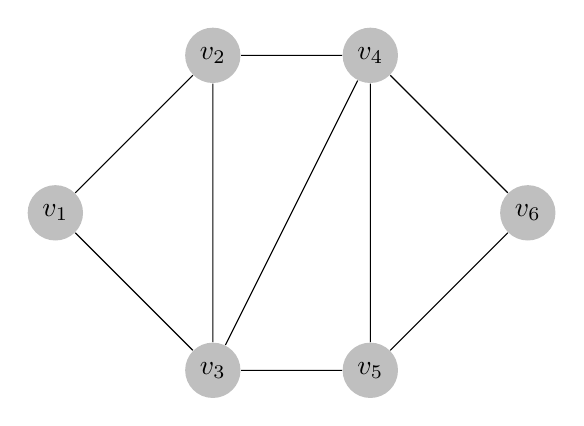
\begin{tikzpicture}
\tikzstyle{vertex}=[circle,fill=black!25,minimum size=20pt,inner sep=0pt]
\node[vertex] (V1) at (0, 2) {$v_1$};
\node[vertex] (V2) at (2, 4) {$v_2$};
\node[vertex] (V3) at (2, 0) {$v_3$};
\node[vertex] (V4) at (4, 4) {$v_4$};
\node[vertex] (V5) at (4, 0) {$v_5$};
\node[vertex] (V6) at (6, 2) {$v_6$};
\draw (V1) -- (V2) -- (V3) -- (V4) -- (V5) -- (V6) -- (V4) -- (V2);
\draw (V1) -- (V3) -- (V5);
\end{tikzpicture}
\end{center}

We wish to know if it is possible to color $G$ using at most $3$ colors. Thus we make $6$ courses, one for each node in $V(G)$. Each course $v_i$ will have a single class, call it $c_i$, and will have three possible starting dates, $\{1, 2, 3\}$.

For every edge in $E(G)$, we will add a single professor. Thus, if we label the edges as such

$$
E(G) = \{(v_1, v_2), (v_2, v_3), (v_3, v_4), (v_4, v_5), (v_5, v_6), (v_4, v_6), (v_2, v_4), (v_1, v_3), (v_3, v_5)\}
$$

then since $|E(G)| = 9$, we will have $9$ professors, $p_1, p_2, \dots, p_9$.

$p_i$ is available on days $\{1, 2, 3\}$, and his only possible role is $i$.

For every edge $e_k = (u, v)$, then, we will add a restriction to our instance: that $p_k$ needs to be present at $u$'s class and $v$'s class. Recall that $\max(c, n, t)$ and $\min(c, n, t)$ were the maximum and minimum number of professors on roles $t$ which were needed on the $n$th class of course $c$.

For readability, we will note $\Gamma(i)$ the types of roles needed for $c_i$'s only class, and we will identify a role with the only professor that can fill that role. That is, $p_k \in \Gamma(i)$ means $\min(i, 1, k) = \max(i, 1, k) = 1$.

\newcommand{\restrict}[3]{\item Since $e_#3 = (v_#1, v_#2) \in E(G)$, $p_#3 \in \Gamma(#1)$, $p_#3 \in \Gamma(#2)$.}

\begin{itemize}
\restrict{1}{2}{1}
\restrict{2}{3}{2}
\restrict{3}{4}{3}
\item $\vdots$
%\restrict{4}{5}{4}
%\restrict{5}{6}{5}
%\restrict{4}{6}{6}
%\restrict{2}{4}{7}
%\restrict{1}{3}{8}
\restrict{3}{5}{9}
\end{itemize}

When we solve this instance, we will get a set of starting days, one for each of the courses, each starting day being one of $\{1, 2, 3\}$.

Take $e_9 = (v_3, v_5)$ for example. Since $p_9 \in \Gamma(3) \cap \Gamma(5)$, and there is only one professor with role $9$, it can't be the case that both $c_3$ and $c_5$ fall on the same day, since $p_9$ would have to be teaching them both in the same day, which is not valid. Thus, course $v_3$ and $v_5$ must have different starting dates, making $c_3$ and $c_5$ fall on different days.

The same holds for every edge in $E(G)$. Thus, if we color a node by its starting date, one valid solution for our instance is the following assignment of starting dates:

\begin{itemize}
\item $v_1$ and $v_4$ start on day $1$.
\item $v_2$ and $v_5$ start on day $2$.
\item $v_3$ and $v_6$ start on day $3$.
\end{itemize}

This yields the following coloring:

\begin{center}
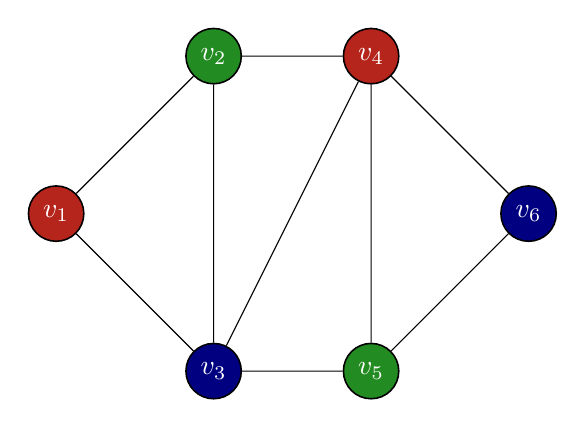
\begin{tikzpicture}
\tikzstyle{vertex}=[circle,fill=black!25,minimum size=20pt,inner sep=0pt, line width=0.2mm, draw=black, text=white]
\node[vertex, fill=BrickRed] (V1) at (0, 2) {$v_1$};
\node[vertex, fill=ForestGreen] (V2) at (2, 4) {$v_2$};
\node[vertex, fill=NavyBlue, text=white] (V3) at (2, 0) {$v_3$};
\node[vertex, fill=BrickRed] (V4) at (4, 4) {$v_4$};
\node[vertex, fill=ForestGreen] (V5) at (4, 0) {$v_5$};
\node[vertex, fill=NavyBlue, text=white] (V6) at (6, 2) {$v_6$};
\draw (V1) -- (V2) -- (V3) -- (V4) -- (V5) -- (V6) -- (V4) -- (V2);
\draw (V1) -- (V3) -- (V5);
\end{tikzpicture}
\end{center}

Thus we obtain a valid 3-coloring of $G$. This shows that 3-COLORING $\le_P$ TIMETABLING, thus TIMETABLING is in \nph, since 3-COLORING is in \nph.

\subsection{Algorithm}

\begin{codebox}

\end{codebox}
